\poczatekwykladu{10}

\section{Przybliżanie funkcjami prostymi}
\label{sec:przyblizanie-funkcjami-prostymi}

W dowodzie addytywności całki funkcji nieujemnych wykorzystamy
przybliżenia od dołu przez funkcje proste. Najpierw skonstruujemy taki
ciąg dla dowolnej funkcji z~$\mathrm{MN}$, a następnie przejdziemy
do granicy pod znakiem całki.

\begin{twierdzenie}[Przybliżenie od dołu]
\label{tw:przyblizanie-funkcjami-prostymi}
Jeżeli $f\in\mathrm{MN}$, to istnieje ciąg $(s_n)$ funkcji
z~$\mathrm{PMN}$ taki, że w każdym punkcie $X$
\[
  0\leq s_1\leq s_2\leq\cdots,\qquad \lim_{n\to\infty}s_n=f.
\]
Piszemy wówczas $s_n\uparrow f$.
\end{twierdzenie}

\begin{proof}
Dla $n\geq1$ obcinamy wartości $f$ na wysokości $n$, a poniżej $n$
dzielimy przedział wartości na odcinki długości $2^{-n}$. Niech
\begin{align*}
  F_n&=\{x\in X:f(x)\geq n\},\\
  E_{n,i}&=\left\{x\in X:\frac{i}{2^n}\leq f(x)
               <\frac{i+1}{2^n}\right\},
               \qquad i=0,1,\ldots,n2^n-1.
\end{align*}
Zbiory te są mierzalne, parami rozłączne i pokrywają $X$. Definiujemy
\begin{equation}
  s_n(x)=
  \begin{cases}
    \dfrac{i}{2^n}, & x\in E_{n,i},\\[4pt]
    n, & x\in F_n.
  \end{cases}
  \label{eq:dyadyczne-przyblizenie}
\end{equation}
Funkcja $s_n$ przyjmuje co najwyżej $n2^n+1$ wartości i należy
do~$\mathrm{PMN}$. Na każdym ze zbiorów $E_{n,i}$ wybieramy lewy koniec
przedziału wartości, więc $s_n\leq f$. Ilustruje to
rysunek~\ref{fig:przyblizenie-dyadyczne}.

Gdy $f(x)<+\infty$, możemy zapisać
\[
  s_n(x)=\min\bigl\{n,2^{-n}\lfloor 2^n f(x)\rfloor\bigr\}.
\]
Węzły podziału o kroku $2^{-n}$ pozostają w podziale o kroku
$2^{-(n+1)}$, zatem zaokrąglenie w dół może tylko wzrosnąć. Wysokość
obcięcia także rośnie, więc $s_n(x)\leq s_{n+1}(x)$. Dla $n>f(x)$
mamy $0\leq f(x)-s_n(x)<2^{-n}$, co daje zbieżność do $f(x)$.
Gdy $f(x)=+\infty$, mamy $s_n(x)=n$ dla każdego $n$ i również
$s_n(x)\uparrow f(x)$.
\end{proof}

\begin{figure}[htbp]
  \centering
  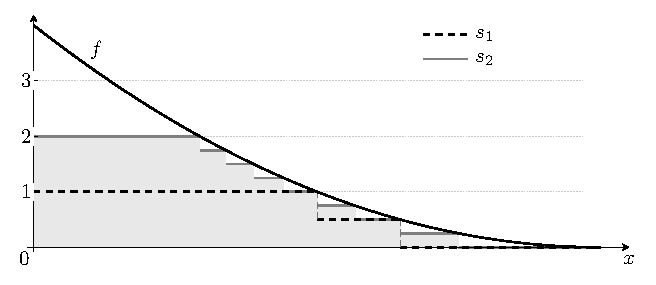
\includegraphics[width=0.73\textwidth]{przyblizenie-dyadyczne.pdf}
  \caption{Przybliżenia $s_1$ i $s_2$ od dołu z krokami odpowiednio $1/2$ i $1/4$.}
  \label{fig:przyblizenie-dyadyczne}
\end{figure}

\section{Zbieżność monotoniczna i addytywność}
\label{sec:zbieznosc-monotoniczna}

\begin{twierdzenie}[Lebesgue'a o zbieżności monotonicznej, Beppo Levi]
\label{tw:zbieznosc-monotoniczna}
Jeżeli $f_n\in\mathrm{MN}$ i $f_n\uparrow f$ punktowo na $X$,
to $f\in\mathrm{MN}$ oraz
\begin{equation}
  \lim_{n\to\infty}\int_X f_n\,d\mu=\int_X f\,d\mu.
  \label{eq:zbieznosc-monotoniczna}
\end{equation}
Ciąg całek po lewej stronie jest niemalejący. Równość zachodzi także,
gdy $f\in\mathrm{MN}$ i $f_n\uparrow f$ prawie wszędzie.
\end{twierdzenie}

\begin{uwaga}
\label{uw:calka-a-zbior-miary-zero}
Punktowa granica funkcji mierzalnych jest mierzalna, a tutaj także
nieujemna. Wersję dla zbieżności prawie wszędzie otrzymamy przez
wyzerowanie $f_n$ i $f$ na wspólnym zbiorze wyjątkowym.

Jeżeli $N\in\mathcal F$ i $\mu(N)=0$, to dla $s\in\mathrm{PMN}$ całki
$s$ i $s\mathbf{1}_{X\setminus N}$ są równe. W postaci kanonicznej
usunięcie $N$ z~poziomic odpowiadających dodatnim wartościom
zachowuje ich miary. Jeżeli $s\leq f$, to $s\mathbf{1}_{X\setminus N}
\leq f\mathbf{1}_{X\setminus N}$. Z tego i z monotoniczności całki
wynika przez supremum w~\eqref{eq:calka-nieujemnej-supremum}, że
wyzerowanie $f\in\mathrm{MN}$ na $N$ zachowuje jej całkę.
\end{uwaga}

\begin{wniosek}
\label{wn:calka-granica-calk-prostych}
Jeżeli $s_n\in\mathrm{PMN}$ i $s_n\uparrow f$ punktowo na $X$, to
\[
  \int_X f\,d\mu=\lim_{n\to\infty}\int_X s_n\,d\mu.
\]
Dla każdego $f\in\mathrm{MN}$ taki ciąg istnieje na mocy
twierdzenia~\ref{tw:przyblizanie-funkcjami-prostymi}.
\end{wniosek}

\begin{proof}[Dowód punktu 3) twierdzenia~\ref{tw:wlasnosci-calki-nieujemnej}]
Niech $f,g\in\mathrm{MN}$. Wybieramy $s_n,t_n\in\mathrm{PMN}$ takie,
że $s_n\uparrow f$ i $t_n\uparrow g$. Wówczas $s_n+t_n$ też należy
do~$\mathrm{PMN}$ i $s_n+t_n\uparrow f+g$. Korzystając z
wniosku~\ref{wn:calka-granica-calk-prostych} i z addytywności całki
funkcji prostych, otrzymujemy
\begin{align*}
  \int_X(f+g)\,d\mu
  &=\lim_{n\to\infty}\int_X(s_n+t_n)\,d\mu\\
  &=\lim_{n\to\infty}\left(\int_X s_n\,d\mu+\int_X t_n\,d\mu\right)\\
  &=\int_X f\,d\mu+\int_X g\,d\mu.
\end{align*}
Przejście do granicy sumy jest poprawne także dla granicy $+\infty$,
ponieważ oba składniki są nieujemne.
\end{proof}

\section{Całka funkcji nieujemnej po zbiorze}
\label{sec:calka-nieujemnej-po-zbiorze}

\begin{definicja}
\label{def:calka-nieujemnej-po-zbiorze}
Dla $f\in\mathrm{MN}$ i $E\in\mathcal F$ kładziemy
\[
  \int_E f\,d\mu=\int_X f\mathbf{1}_E\,d\mu.
\]
Funkcja $f\mathbf{1}_E$ jest równa $f$ na $E$ i zero poza $E$.
Jest mierzalna i nieujemna. Gdy pomijamy zbiór pod znakiem całki,
mamy na myśli całkę po $X$.
\end{definicja}

\begin{fakt}
\label{fakt:calka-nieujemnej-po-rozlacznych}
Jeżeli $f\in\mathrm{MN}$, $E,F\in\mathcal F$ i $E\cap F=\varnothing$, to
\[
  \int_{E\cup F} f\,d\mu=\int_E f\,d\mu+\int_F f\,d\mu.
\]
\end{fakt}

\begin{proof}
Z rozłączności wynika $\mathbf{1}_{E\cup F}=\mathbf{1}_E+\mathbf{1}_F$.
Zatem
\[
  \int_{E\cup F} f\,d\mu
  =\int_X(f\mathbf{1}_E+f\mathbf{1}_F)\,d\mu
  =\int_E f\,d\mu+\int_F f\,d\mu
\]
na mocy addytywności całki funkcji nieujemnej.
\end{proof}

\section{Całka funkcji mierzalnej: etap trzeci}
\label{sec:calka-funkcji-etap-trzeci}

\begin{definicja}[Część dodatnia i część ujemna]
\label{def:czesc-dodatnia-i-ujemna}
Dla $f\colon X\to\Rbar$ część dodatnią i część ujemną określamy wzorami
\begin{align*}
  f^+(x)&=\max\{f(x),0\}
         =f(x)\mathbf{1}_{\{f\geq0\}}(x),\\
  f^-(x)&=\max\{-f(x),0\}=-\min\{f(x),0\}
         =-f(x)\mathbf{1}_{\{f\leq0\}}(x).
\end{align*}
Iloczyn przez funkcję charakterystyczną przyjmuje poza jej zbiorem
wartość zero także dla nieskończonego $f(x)$. Obie części są
nieujemne i w każdym punkcie przynajmniej jedna jest zerowa.
W szczególności
\begin{equation}
  f=f^+-f^-,\qquad |f|=f^++f^-.
  \label{eq:rozklad-na-czesci}
\end{equation}
\end{definicja}

Na rysunku~\ref{fig:czesci-funkcji} część $f^-$ powstaje przez odbicie
ujemnego fragmentu wykresu $f$ względem osi poziomej.

\begin{figure}[htbp]
  \centering
  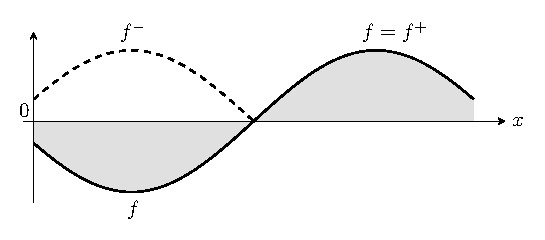
\includegraphics[width=0.58\textwidth]{czesci-funkcji.pdf}
  \caption{Funkcja $f$ oraz jej części dodatnia $f^+$ i ujemna $f^-$.}
  \label{fig:czesci-funkcji}
\end{figure}

\begin{fakt}
\label{fakt:mierzalnosc-czesci-funkcji}
Funkcja $f$ jest mierzalna wtedy i tylko wtedy, gdy obie funkcje $f^+$
i $f^-$ są mierzalne.
\end{fakt}

\begin{proof}
Dla mierzalnego $f$ obie części są mierzalne jako złożenia z ciągłymi
funkcjami $t\mapsto\max\{t,0\}$ i $t\mapsto\max\{-t,0\}$ na~$\Rbar$.
W drugą stronę, dla $a\geq0$ mamy $\{f>a\}=\{f^+>a\}$, zaś dla $a<0$
mamy $\{f>a\}=\{f^-<-a\}$. Oba rodzaje zbiorów są mierzalne.
\end{proof}

\begin{definicja}[Całka funkcji mierzalnej]
\label{def:calka-funkcji-mierzalnej}
Jeżeli $f$ jest mierzalna i co najmniej jedna z całek $\int_X f^+\,d\mu$,
$\int_X f^-\,d\mu$ jest skończona, definiujemy
\begin{equation}
  \int_X f\,d\mu=\int_X f^+\,d\mu-\int_X f^-\,d\mu.
  \label{eq:calka-przez-czesci}
\end{equation}
Gdy obie całki części są nieskończone, całka z $f$ pozostaje
nieokreślona.
\end{definicja}

\begin{definicja}[Całkowalność]
\label{def:calkowalnosc}
Funkcja mierzalna $f$ jest całkowalna, gdy
\[
  \int_X f^+\,d\mu<+\infty\qquad\text{i}\qquad
  \int_X f^-\,d\mu<+\infty.
\]
Równoważnie, całka $\int_X f\,d\mu$ istnieje i jest skończona.
Innym równoważnym warunkiem jest $\int_X |f|\,d\mu<+\infty$,
ponieważ z~\eqref{eq:rozklad-na-czesci} i addytywności całki funkcji
nieujemnej wynika
\[
  \int_X |f|\,d\mu=\int_X f^+\,d\mu+\int_X f^-\,d\mu.
\]
\end{definicja}

\begin{fakt}
\label{fakt:modul-calki}
Jeżeli całka $\int_X f\,d\mu$ jest określona, to
\begin{equation}
  \left|\int_X f\,d\mu\right|\leq \int_X|f|\,d\mu.
  \label{eq:modul-calki}
\end{equation}
\end{fakt}

\begin{proof}
Dla skończonych całek obu części mamy
\[
  \left|\int_X f\,d\mu\right|
  =\left|\int_X f^+\,d\mu-\int_X f^-\,d\mu\right|
  \leq\int_X f^+\,d\mu+\int_X f^-\,d\mu
  =\int_X|f|\,d\mu.
\]
Jeżeli dokładnie jedna całka części jest nieskończona,
obie strony~\eqref{eq:modul-calki} są równe $+\infty$.
\end{proof}

\begin{definicja}[Całka i całkowalność na zbiorze]
\label{def:calkowalnosc-na-zbiorze}
Dla mierzalnych $f$ i $E\in\mathcal F$ definiujemy
\[
  \int_E f\,d\mu=\int_X f\mathbf{1}_E\,d\mu,
\]
o ile całka po prawej stronie jest określona. Mówimy, że $f$ jest
całkowalna na $E$, gdy $f\mathbf{1}_E$ jest całkowalna na $X$.
\end{definicja}

\begin{fakt}
\label{fakt:calkowalnosc-na-podzbiorze}
Jeżeli $E,F\in\mathcal F$, $E\subseteq F$ i $f$ jest całkowalna na $F$,
to $f$ jest całkowalna na $E$ i
\[
  \int_E |f|\,d\mu\leq\int_F |f|\,d\mu.
\]
\end{fakt}

\begin{proof}
Z nierówności $|f|\mathbf{1}_E\leq |f|\mathbf{1}_F$ i monotoniczności
całki funkcji nieujemnej otrzymujemy podane oszacowanie. Skończoność
prawej strony daje całkowalność $f$ na $E$.
\end{proof}
